\subsection{Washington}
\begin{figure}[htb!] \centering
\caption{ Current Districts }
\includegraphics[width=5in,height=3in,keepaspectratio]{../maps/WA/static/0_before.png}
\caption{ New Districts (Black Param = 0) }
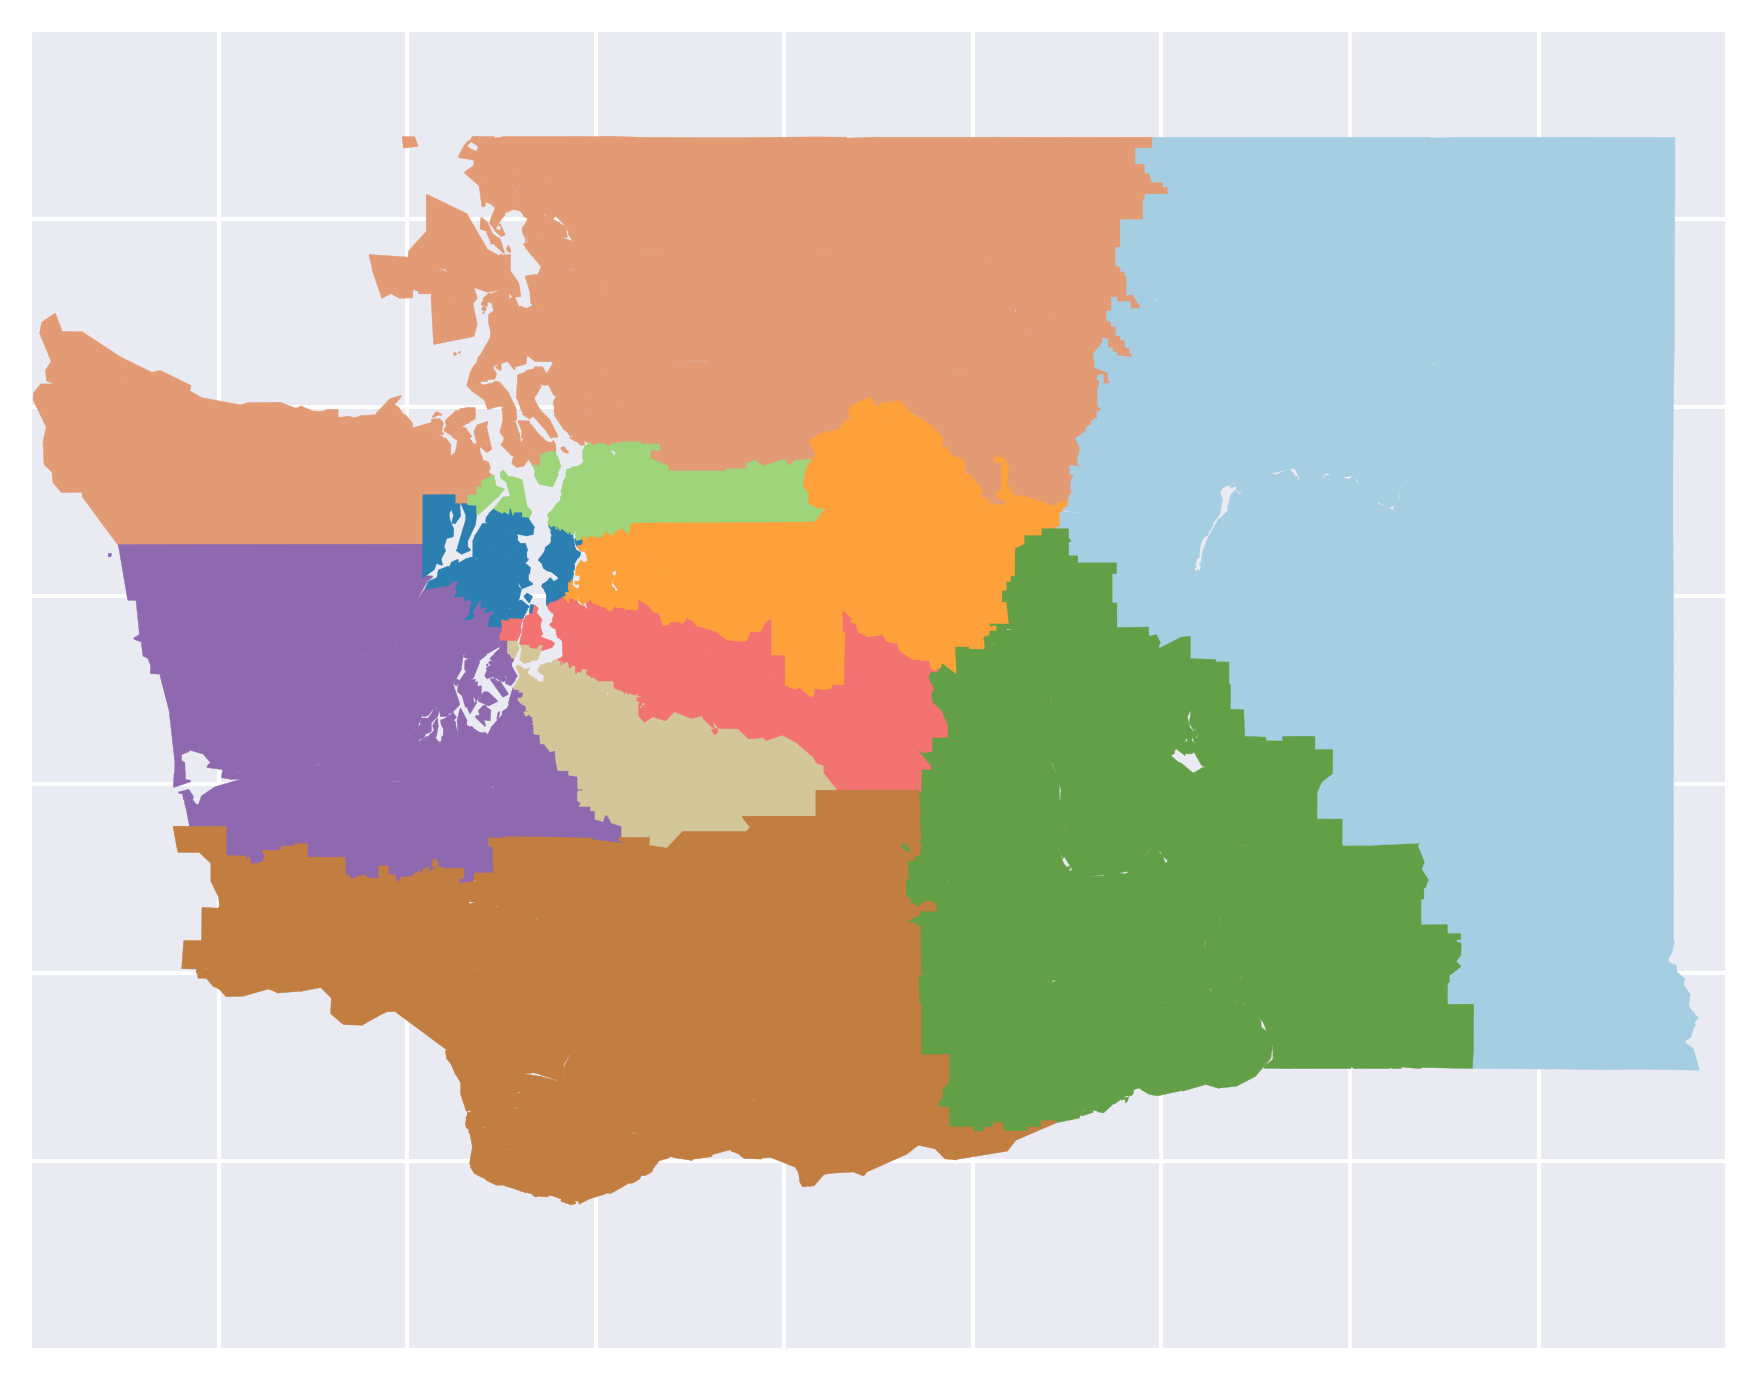
\includegraphics[width=5in,height=3in,keepaspectratio]{../maps/WA/static/0_after.png}
\caption{ New Districts (Black Param = 1) }
\includegraphics[width=5in,height=3in,keepaspectratio]{../maps/WA/static/1_after.png}
\end{figure}

\clearpage
\newpage

\begin{figure}[htb!] \centering
\caption{ Demographics: black population }
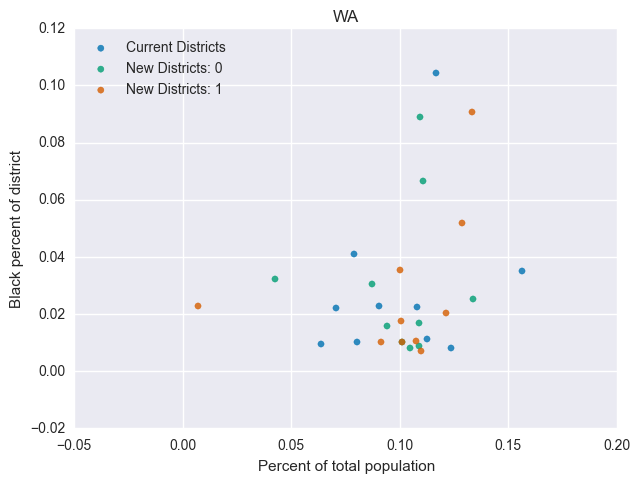
\includegraphics[width=4.5in]{../analysis/WA/analysis_scatter.png}
\caption{ Politics: democratic population (placeholder)}
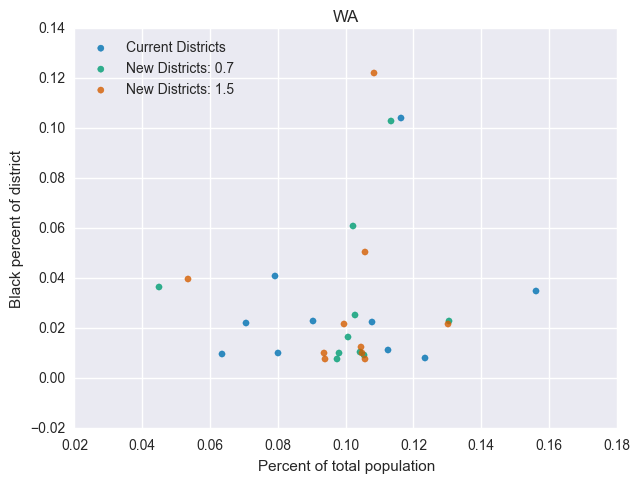
\includegraphics[width=4.5in]{../analysis/WA/analysis_scatter2.png}
\end{figure}

\clearpage
\newpage

\subsection{Florida}
\begin{figure}[htb!] \centering
\caption{ Current Districts }
\includegraphics[width=5in,height=3in,keepaspectratio]{../maps/FL/static/0_before.png}
\caption{ New Districts (Black Param = 0) }
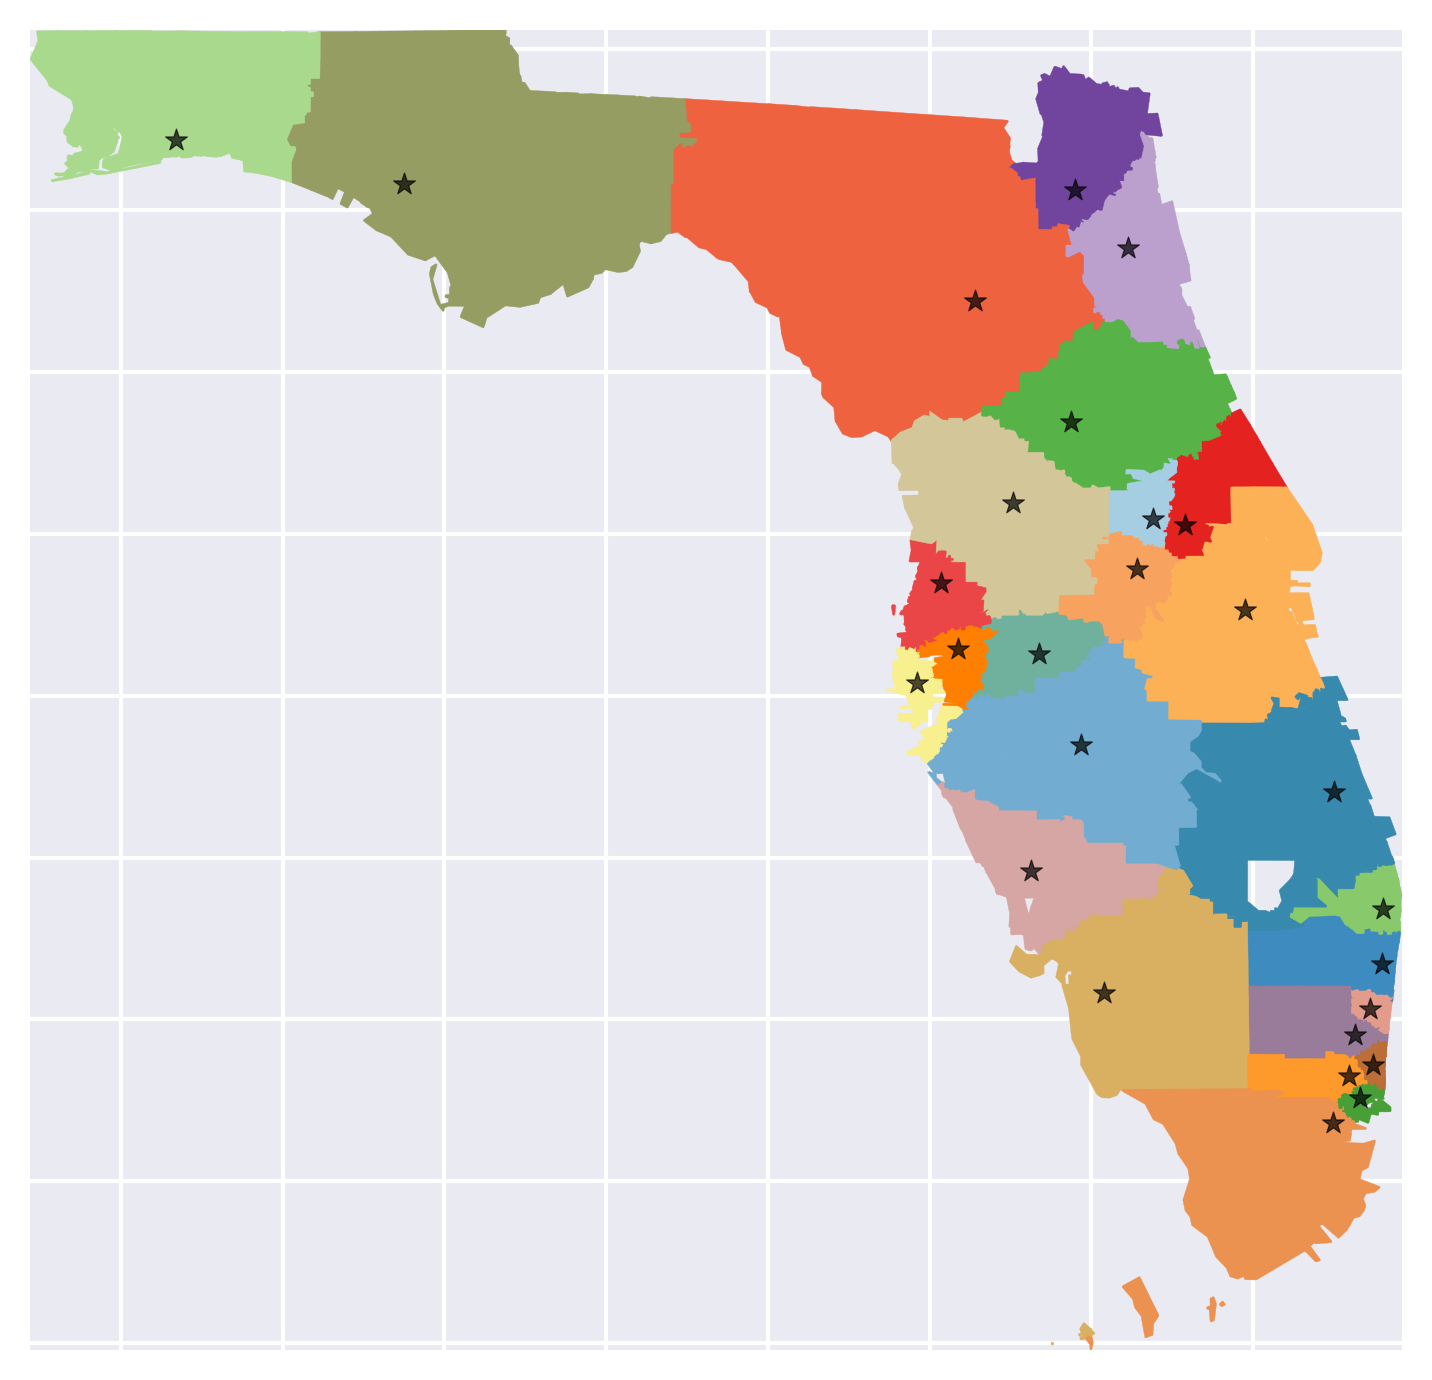
\includegraphics[width=5in,height=3in,keepaspectratio]{../maps/FL/static/0_after.png}
\caption{ New Districts (Black Param = 1) }
\includegraphics[width=5in,height=3in,keepaspectratio]{../maps/FL/static/1_after.png}
\end{figure}

\clearpage
\newpage

\begin{figure}[htb!] \centering
\caption{ Demographics: black population }
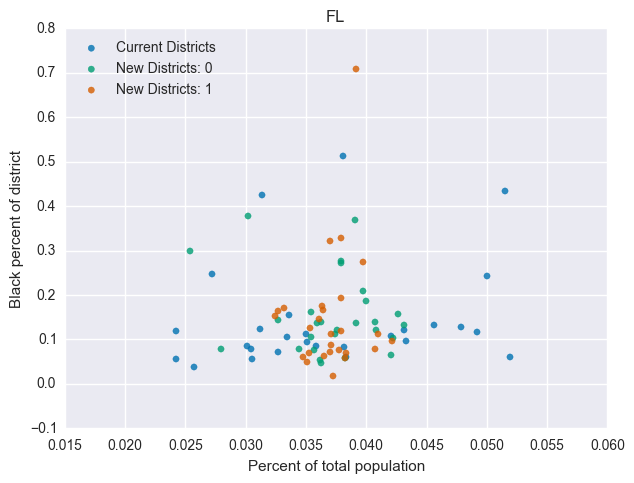
\includegraphics[width=4.5in]{../analysis/FL/analysis_scatter.png}
\caption{ Politics: democratic population (placeholder)}
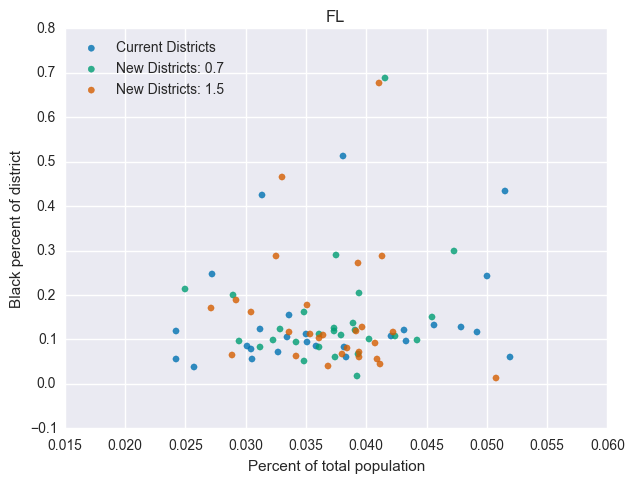
\includegraphics[width=4.5in]{../analysis/FL/analysis_scatter2.png}
\end{figure}

\clearpage
\newpage

\subsection{New Jersey}
\begin{figure}[htb!] \centering
\caption{ Current Districts }
\includegraphics[width=5in,height=3in,keepaspectratio]{../maps/NJ/static/0_before.png}
\caption{ New Districts (Black Param = 0) }
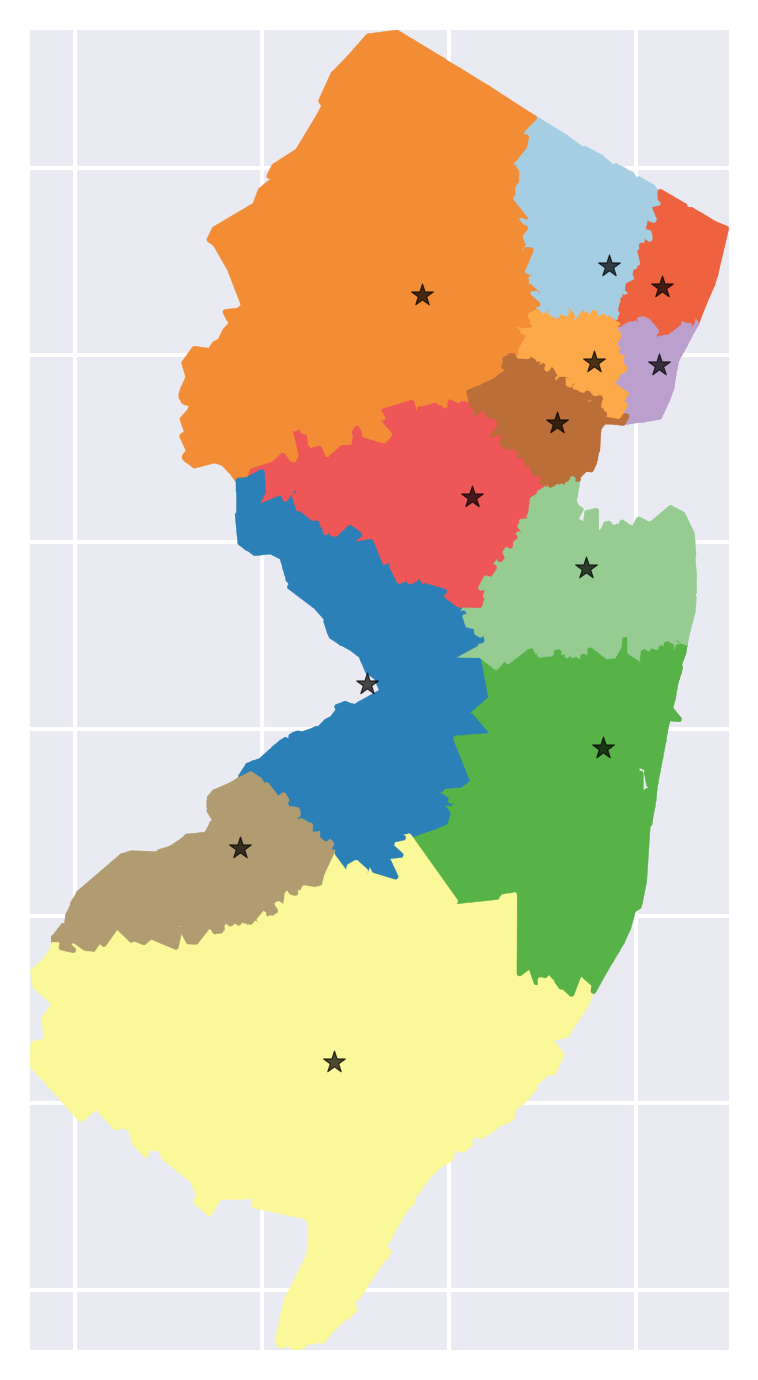
\includegraphics[width=5in,height=3in,keepaspectratio]{../maps/NJ/static/0_after.png}
\caption{ New Districts (Black Param = 1) }
\includegraphics[width=5in,height=3in,keepaspectratio]{../maps/NJ/static/1_after.png}
\end{figure}

\clearpage
\newpage

\begin{figure}[htb!] \centering
\caption{ Demographics: black population }
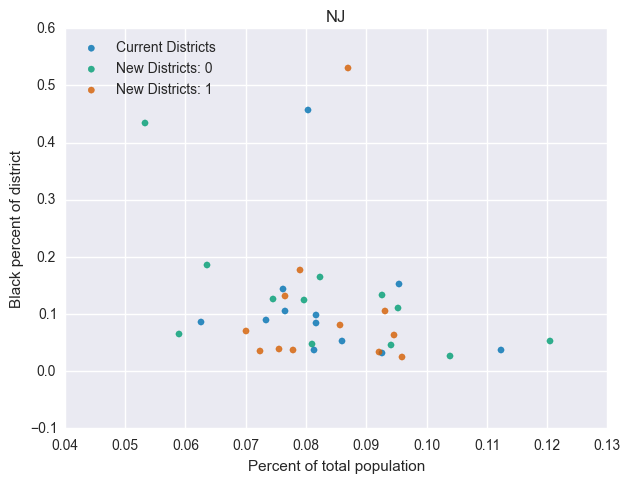
\includegraphics[width=4.5in]{../analysis/NJ/analysis_scatter.png}
\caption{ Politics: democratic population (placeholder)}
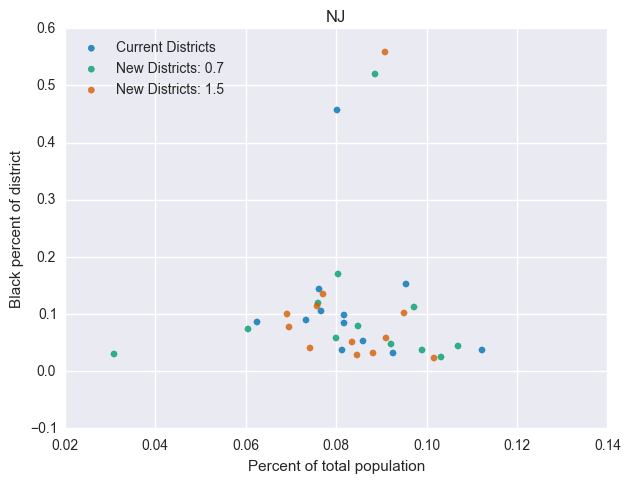
\includegraphics[width=4.5in]{../analysis/NJ/analysis_scatter2.png}
\end{figure}

\clearpage
\newpage

\subsection{Louisiana}
\begin{figure}[htb!] \centering
\caption{ Current Districts }
\includegraphics[width=5in,height=3in,keepaspectratio]{../maps/LA/static/0_before.png}
\caption{ New Districts (Black Param = 0) }
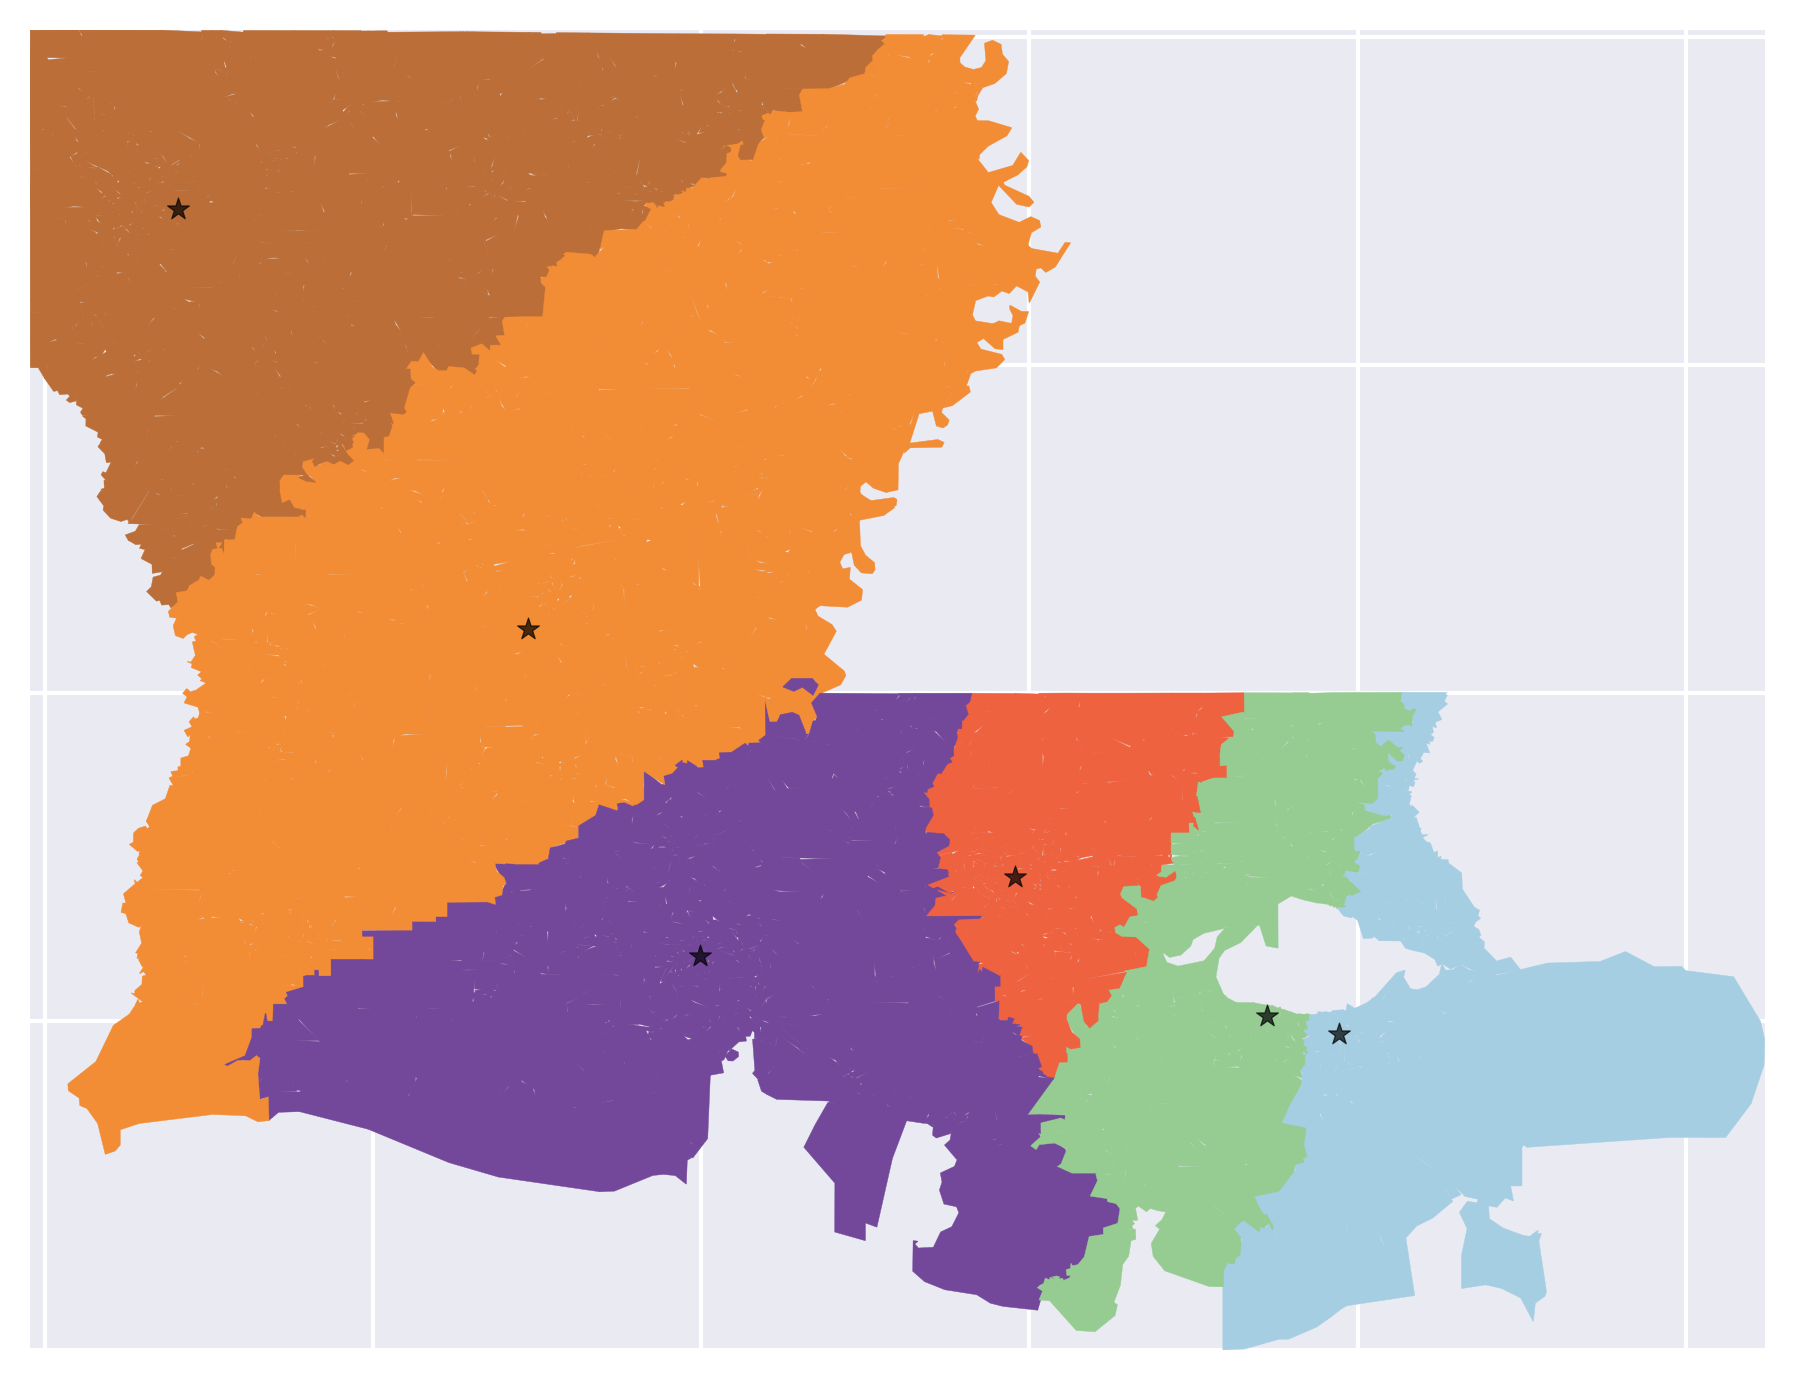
\includegraphics[width=5in,height=3in,keepaspectratio]{../maps/LA/static/0_after.png}
\caption{ New Districts (Black Param = 1) }
\includegraphics[width=5in,height=3in,keepaspectratio]{../maps/LA/static/1_after.png}
\end{figure}

\clearpage
\newpage

\begin{figure}[htb!] \centering
\caption{ Demographics: black population }
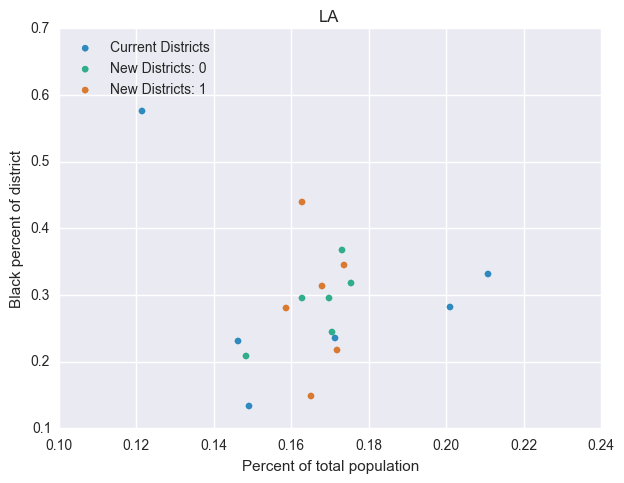
\includegraphics[width=4.5in]{../analysis/LA/analysis_scatter.png}
\caption{ Politics: democratic population (placeholder)}
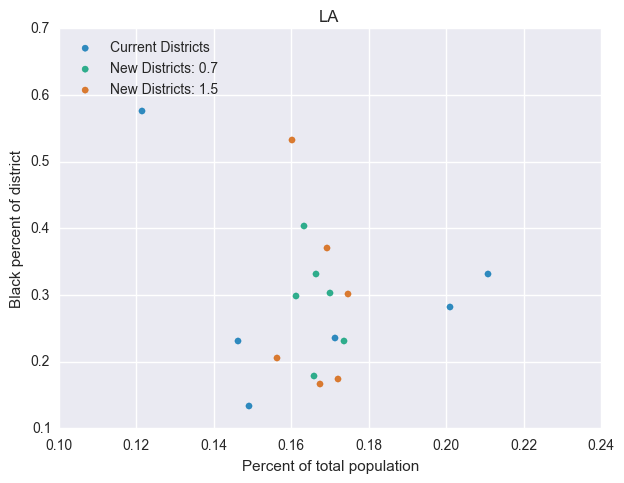
\includegraphics[width=4.5in]{../analysis/LA/analysis_scatter2.png}
\end{figure}

\clearpage
\newpage

\subsection{North Carolina}
\begin{figure}[htb!] \centering
\caption{ Current Districts }
\includegraphics[width=5in,height=3in,keepaspectratio]{../maps/NC/static/0_before.png}
\caption{ New Districts (Black Param = 0) }
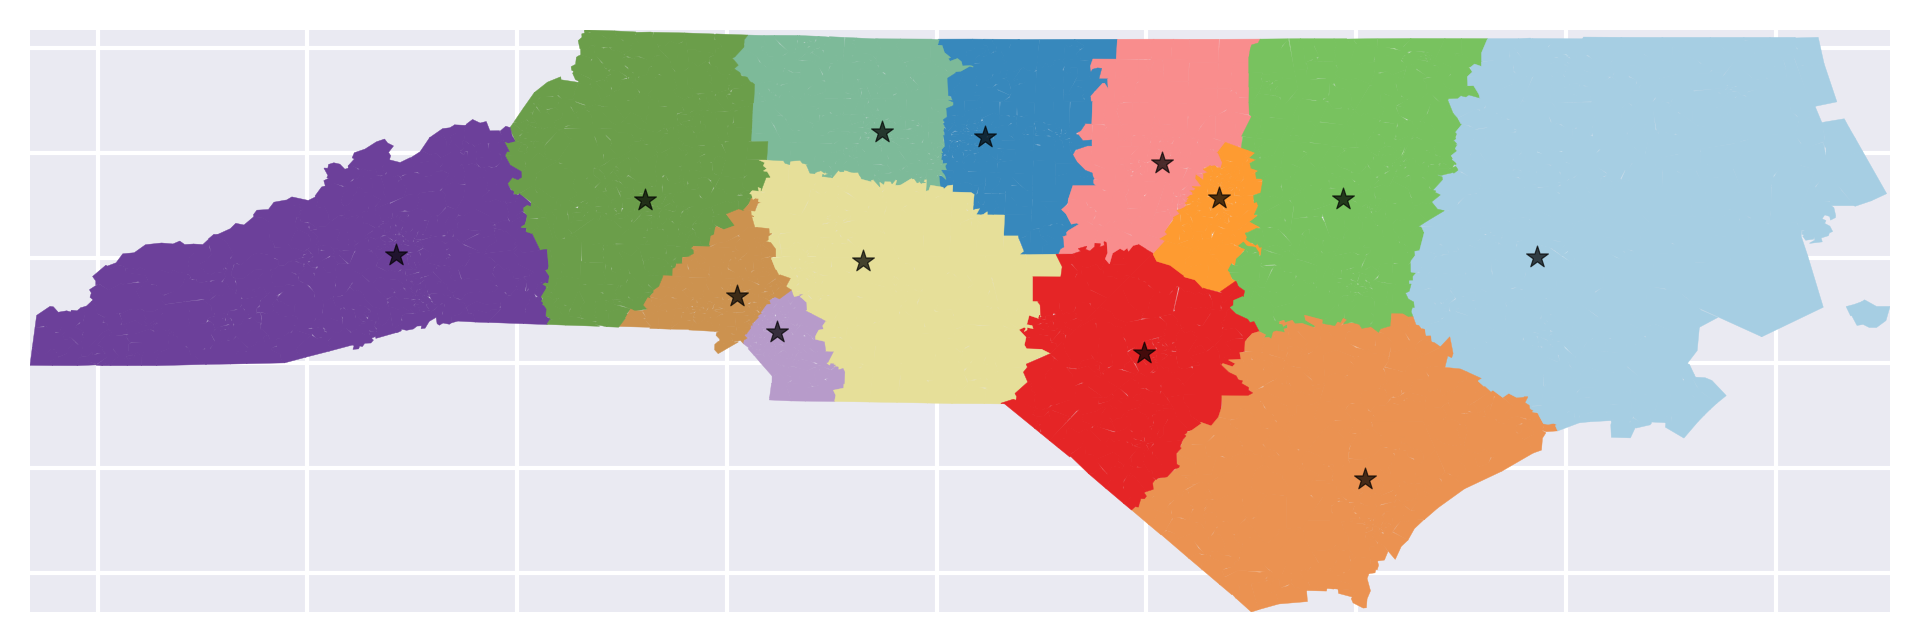
\includegraphics[width=5in,height=3in,keepaspectratio]{../maps/NC/static/0_after.png}
\caption{ New Districts (Black Param = 1) }
\includegraphics[width=5in,height=3in,keepaspectratio]{../maps/NC/static/1_after.png}
\end{figure}

\clearpage
\newpage

\begin{figure}[htb!] \centering
\caption{ Demographics: black population }
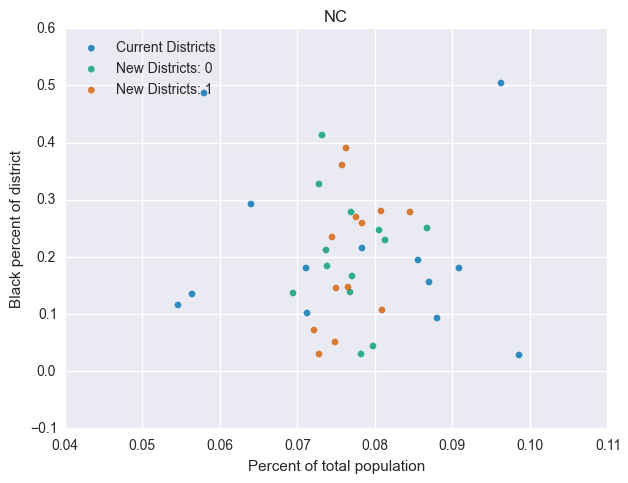
\includegraphics[width=4.5in]{../analysis/NC/analysis_scatter.png}
\caption{ Politics: democratic population (placeholder)}
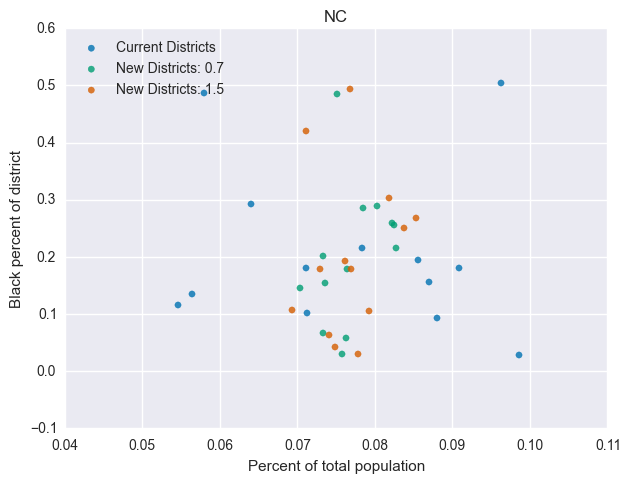
\includegraphics[width=4.5in]{../analysis/NC/analysis_scatter2.png}
\end{figure}

\clearpage
\newpage

\subsection{Tennessee}
\begin{figure}[htb!] \centering
\caption{ Current Districts }
\includegraphics[width=5in,height=3in,keepaspectratio]{../maps/TN/static/0_before.png}
\caption{ New Districts (Black Param = 0) }
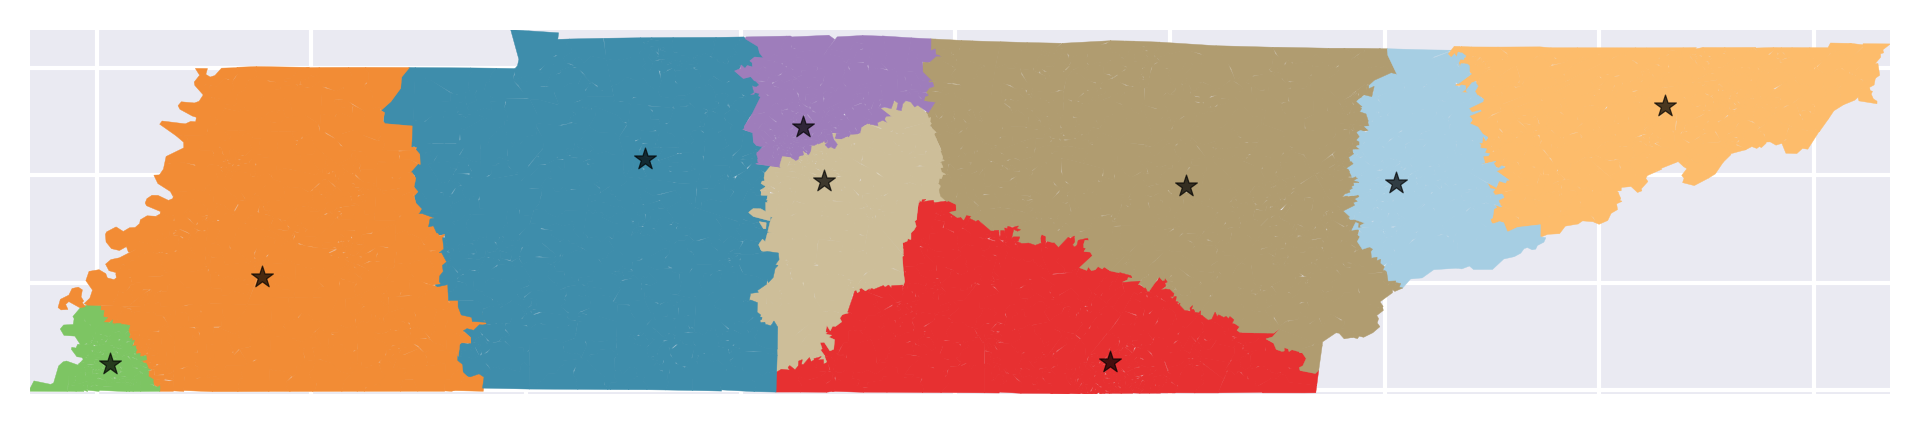
\includegraphics[width=5in,height=3in,keepaspectratio]{../maps/TN/static/0_after.png}
\caption{ New Districts (Black Param = 1) }
\includegraphics[width=5in,height=3in,keepaspectratio]{../maps/TN/static/1_after.png}
\end{figure}

\clearpage
\newpage

\begin{figure}[htb!] \centering
\caption{ Demographics: black population }
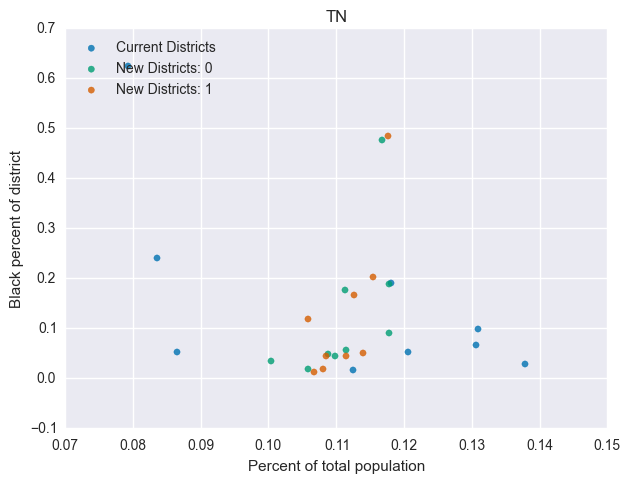
\includegraphics[width=4.5in]{../analysis/TN/analysis_scatter.png}
\caption{ Politics: democratic population (placeholder)}
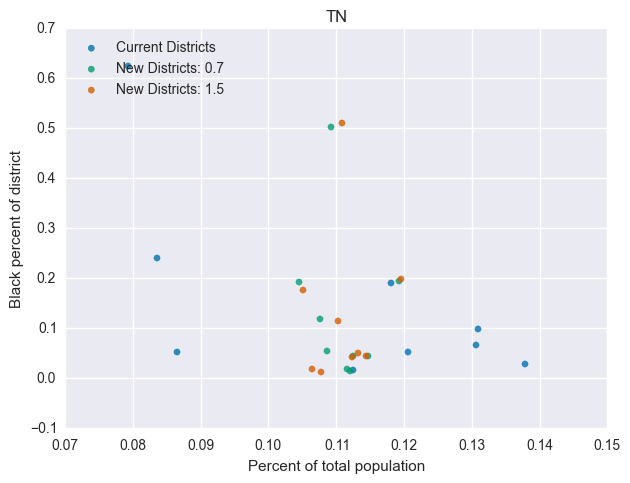
\includegraphics[width=4.5in]{../analysis/TN/analysis_scatter2.png}
\end{figure}

\clearpage
\newpage

\subsection{Pennsylvania}
\begin{figure}[htb!] \centering
\caption{ Current Districts }
\includegraphics[width=5in,height=3in,keepaspectratio]{../maps/PA/static/0_before.png}
\caption{ New Districts (Black Param = 0) }
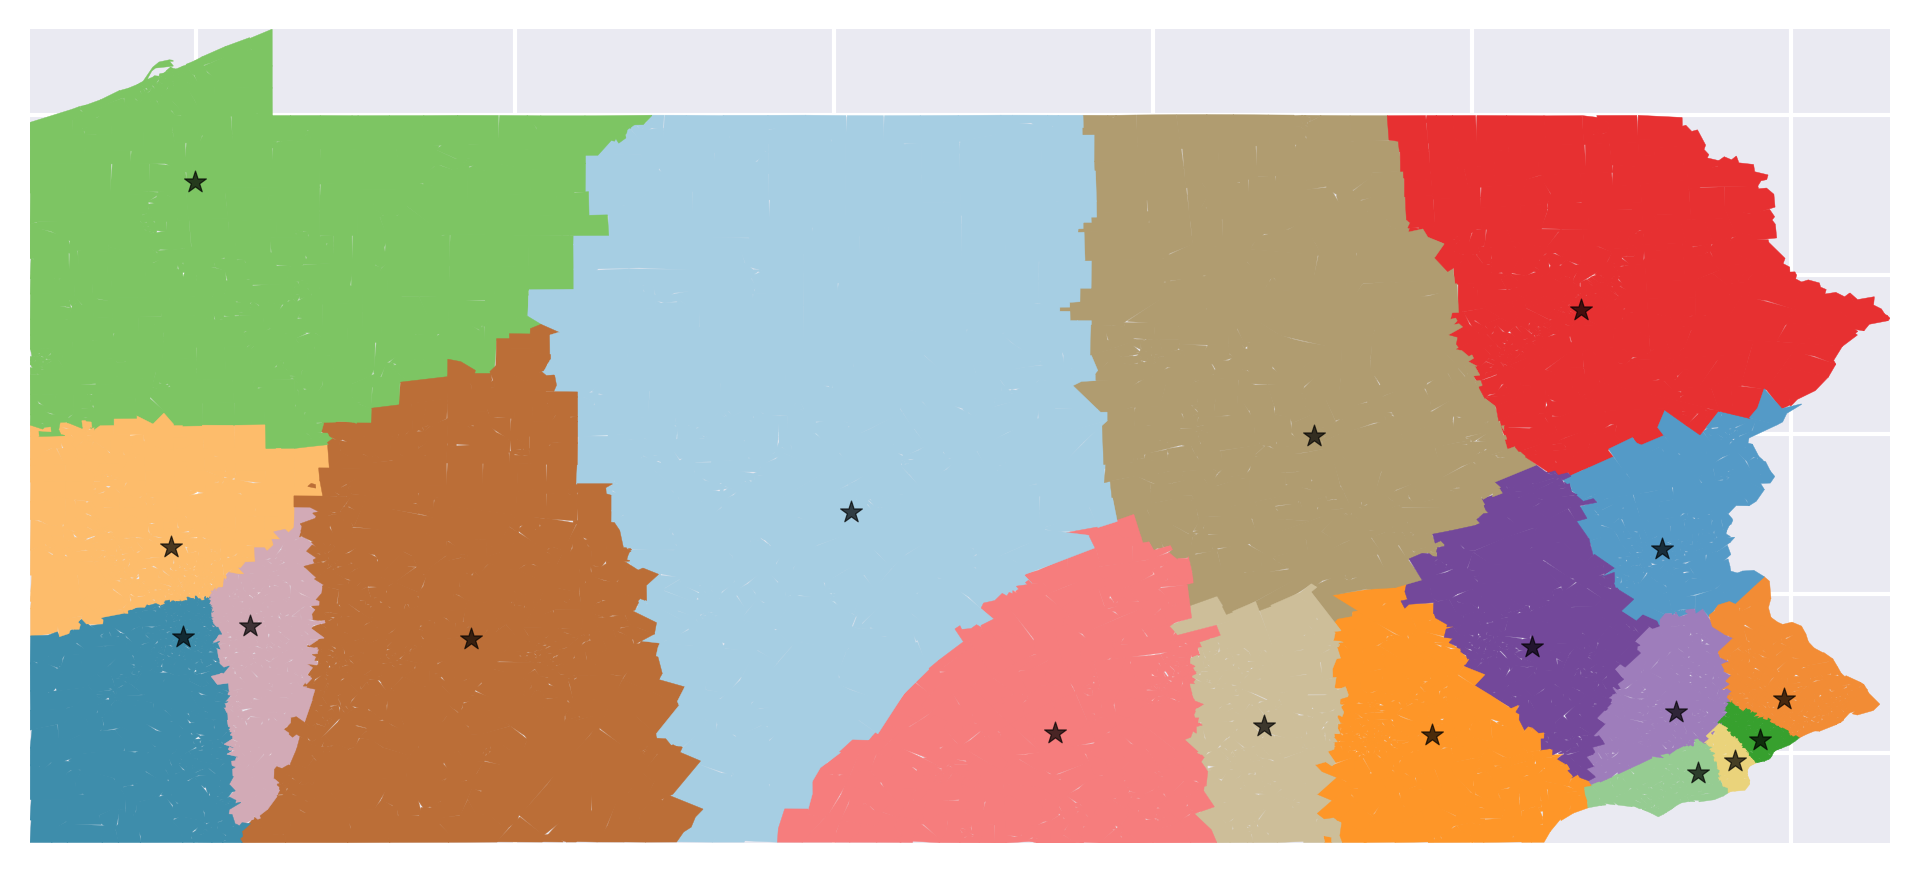
\includegraphics[width=5in,height=3in,keepaspectratio]{../maps/PA/static/0_after.png}
\caption{ New Districts (Black Param = 1) }
\includegraphics[width=5in,height=3in,keepaspectratio]{../maps/PA/static/1_after.png}
\end{figure}

\clearpage
\newpage

\begin{figure}[htb!] \centering
\caption{ Demographics: black population }
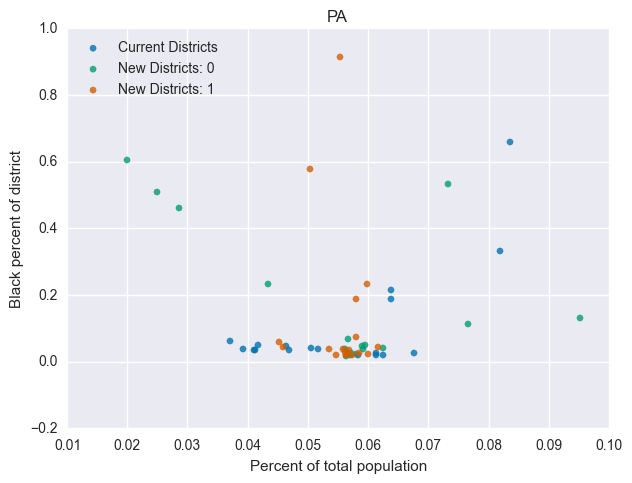
\includegraphics[width=4.5in]{../analysis/PA/analysis_scatter.png}
\caption{ Politics: democratic population (placeholder)}
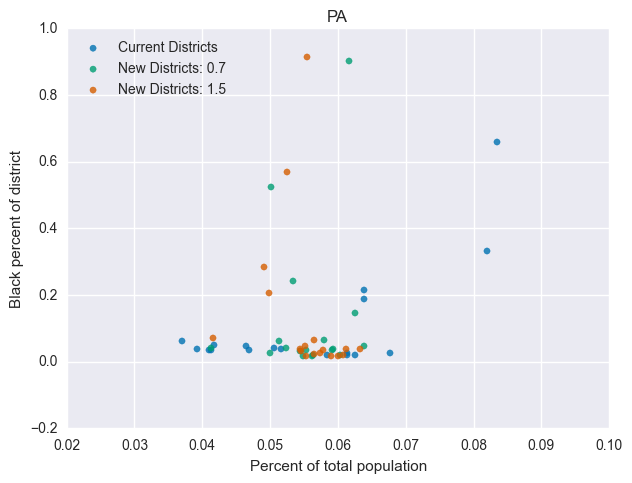
\includegraphics[width=4.5in]{../analysis/PA/analysis_scatter2.png}
\end{figure}

\clearpage
\newpage

\subsection{Virginia}
\begin{figure}[htb!] \centering
\caption{ Current Districts }
\includegraphics[width=5in,height=3in,keepaspectratio]{../maps/VA/static/0_before.png}
\caption{ New Districts (Black Param = 0) }
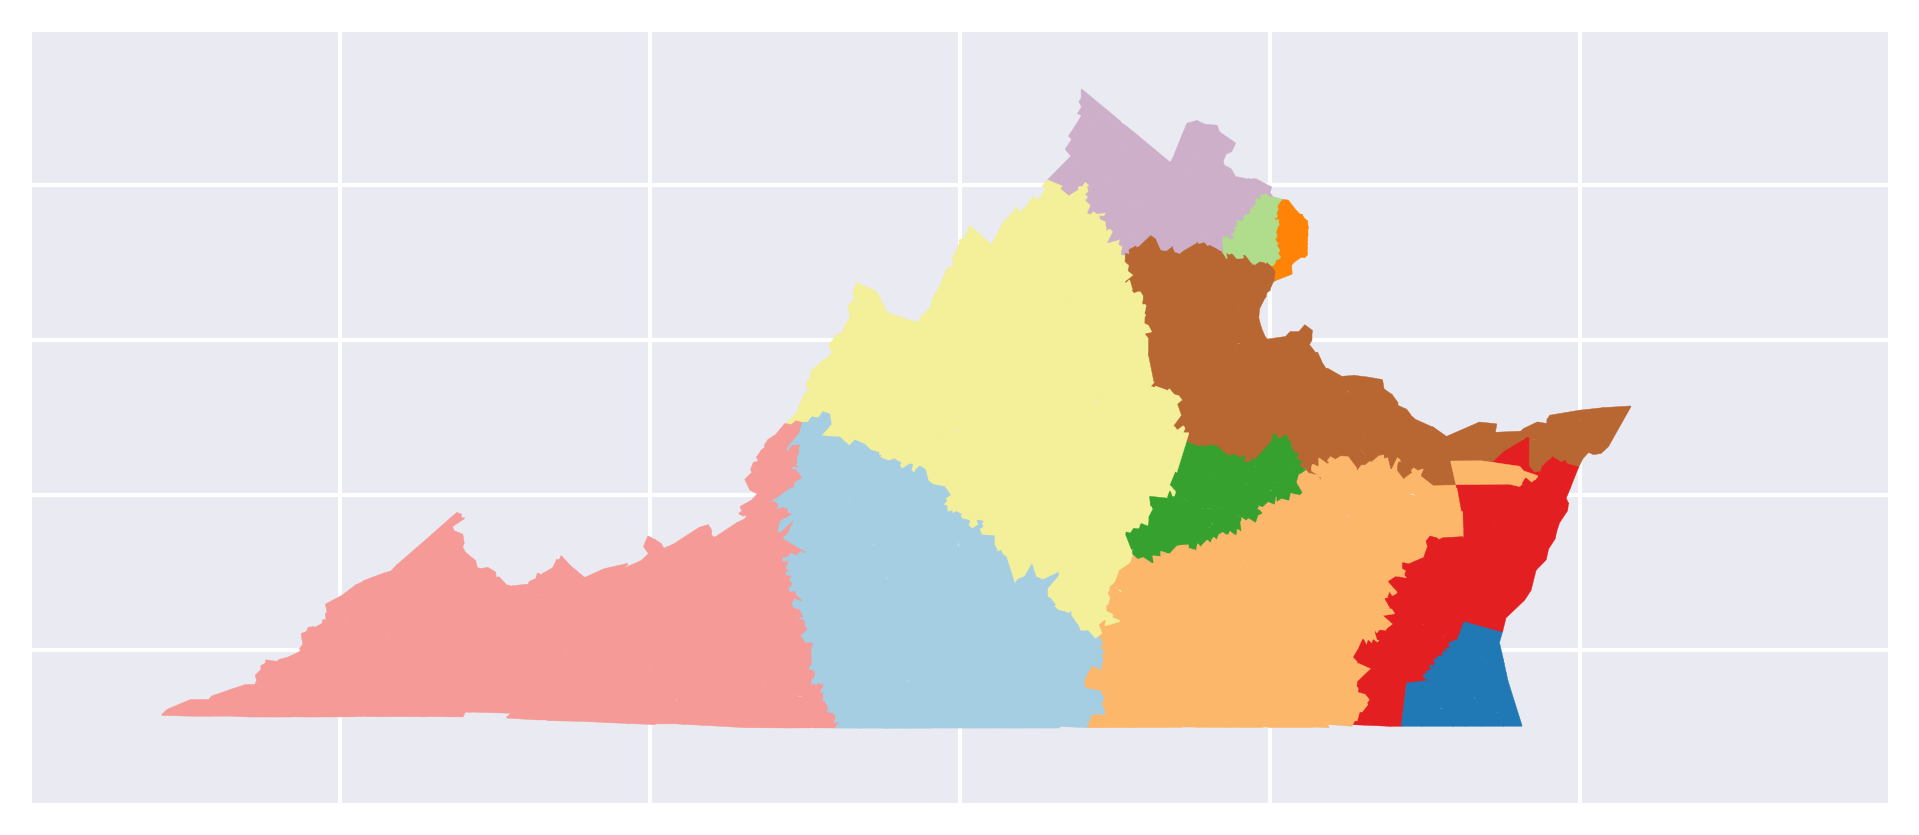
\includegraphics[width=5in,height=3in,keepaspectratio]{../maps/VA/static/0_after.png}
\caption{ New Districts (Black Param = 1) }
\includegraphics[width=5in,height=3in,keepaspectratio]{../maps/VA/static/1_after.png}
\end{figure}

\clearpage
\newpage

\begin{figure}[htb!] \centering
\caption{ Demographics: black population }
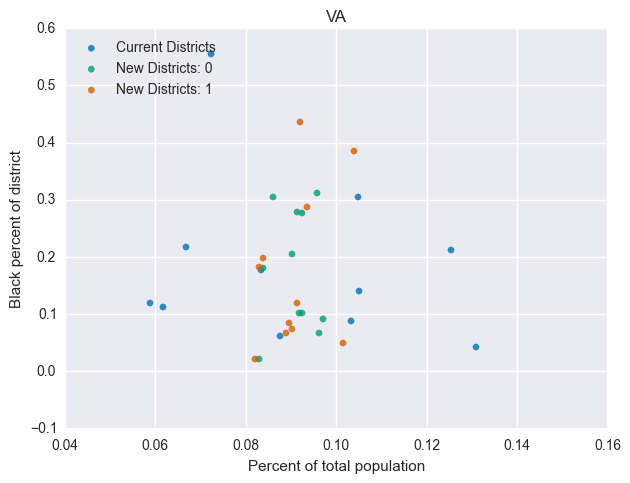
\includegraphics[width=4.5in]{../analysis/VA/analysis_scatter.png}
\caption{ Politics: democratic population (placeholder)}
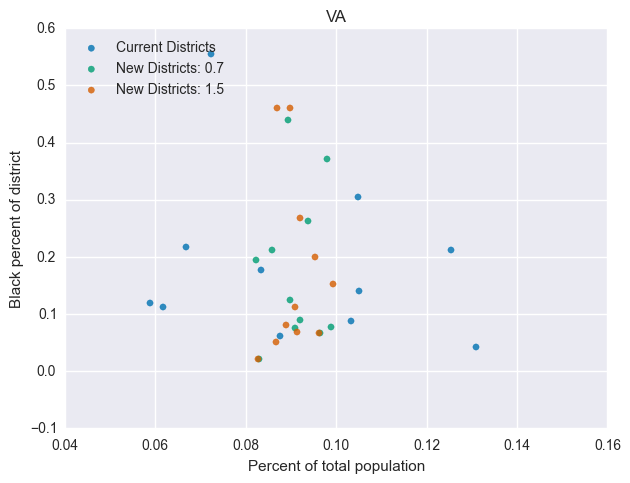
\includegraphics[width=4.5in]{../analysis/VA/analysis_scatter2.png}
\end{figure}

\clearpage
\newpage

\subsection{Colorado}
\begin{figure}[htb!] \centering
\caption{ Current Districts }
\includegraphics[width=5in,height=3in,keepaspectratio]{../maps/CO/static/0_before.png}
\caption{ New Districts (Black Param = 0) }
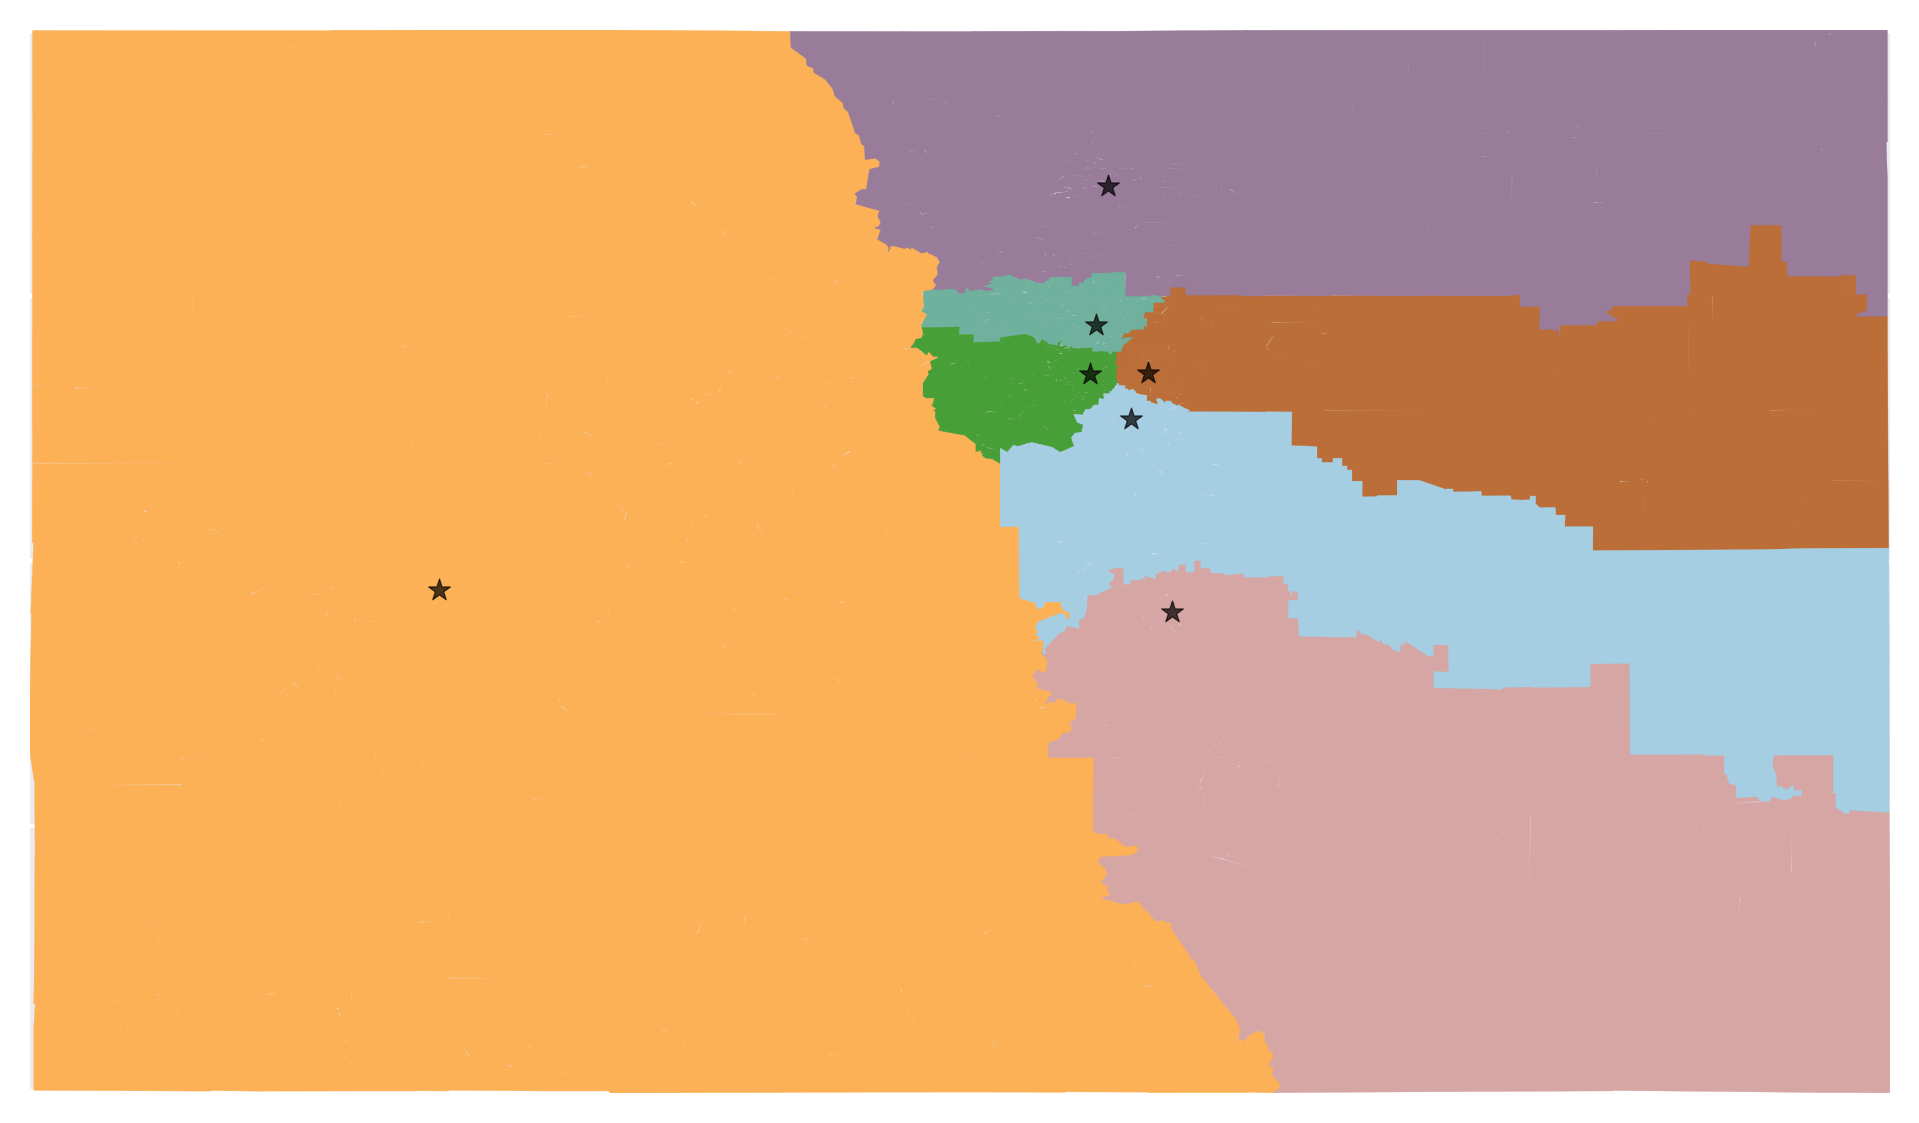
\includegraphics[width=5in,height=3in,keepaspectratio]{../maps/CO/static/0_after.png}
\caption{ New Districts (Black Param = 1) }
\includegraphics[width=5in,height=3in,keepaspectratio]{../maps/CO/static/1_after.png}
\end{figure}

\clearpage
\newpage

\begin{figure}[htb!] \centering
\caption{ Demographics: black population }
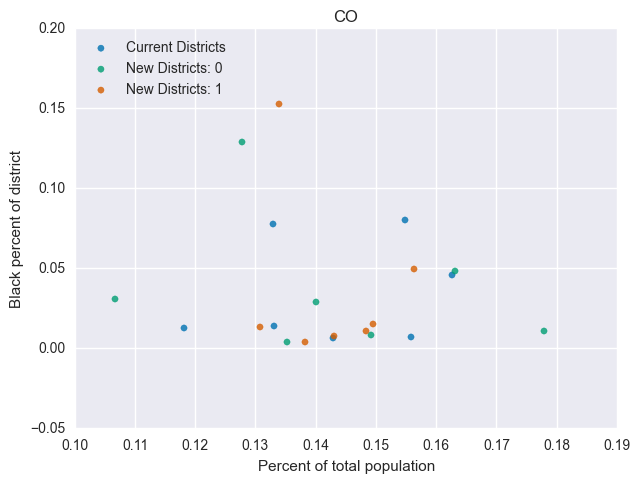
\includegraphics[width=4.5in]{../analysis/CO/analysis_scatter.png}
\caption{ Politics: democratic population (placeholder)}
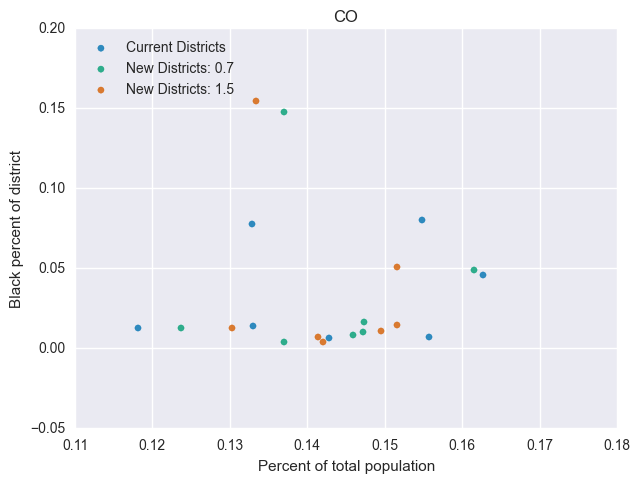
\includegraphics[width=4.5in]{../analysis/CO/analysis_scatter2.png}
\end{figure}

\clearpage
\newpage

\subsection{California}
\begin{figure}[htb!] \centering
\caption{ Current Districts }
\includegraphics[width=5in,height=3in,keepaspectratio]{../maps/CA/static/0_before.png}
\caption{ New Districts (Black Param = 0) }
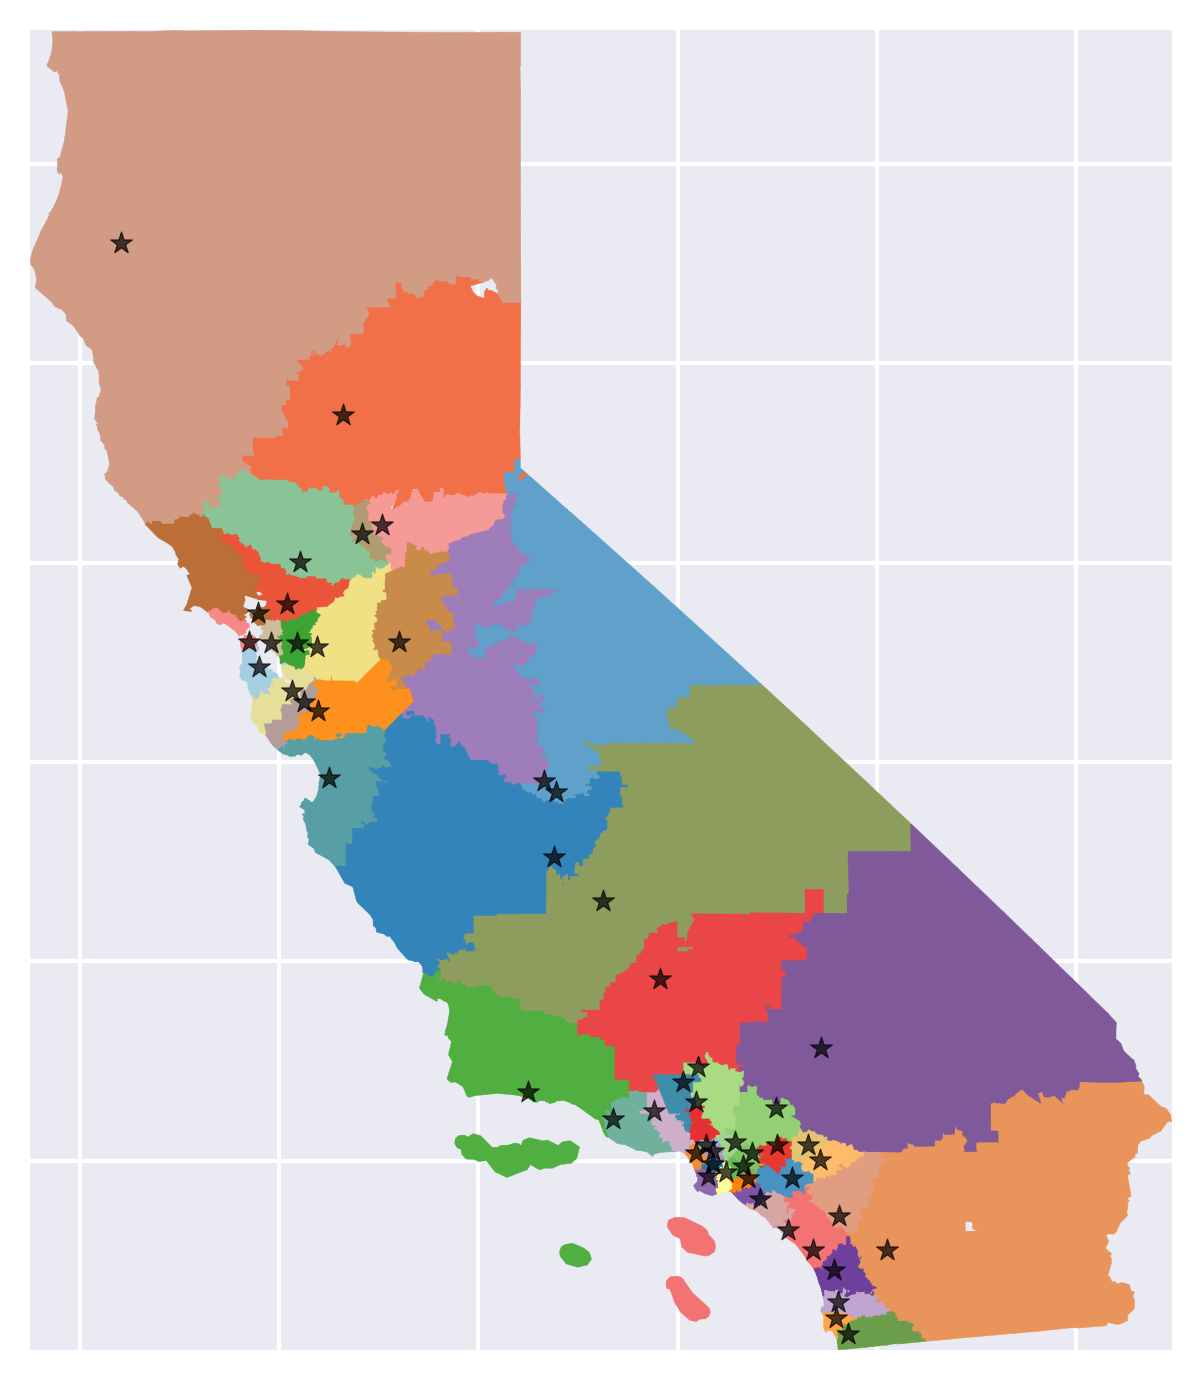
\includegraphics[width=5in,height=3in,keepaspectratio]{../maps/CA/static/0_after.png}
\caption{ New Districts (Black Param = 1) }
\includegraphics[width=5in,height=3in,keepaspectratio]{../maps/CA/static/1_after.png}
\end{figure}

\clearpage
\newpage

\begin{figure}[htb!] \centering
\caption{ Demographics: black population }
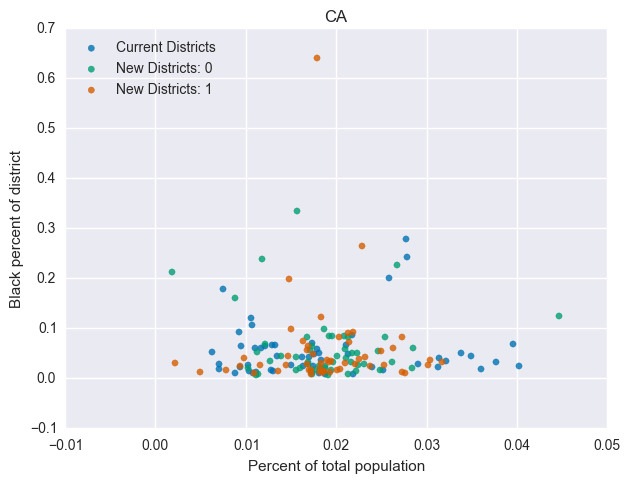
\includegraphics[width=4.5in]{../analysis/CA/analysis_scatter.png}
\caption{ Politics: democratic population (placeholder)}
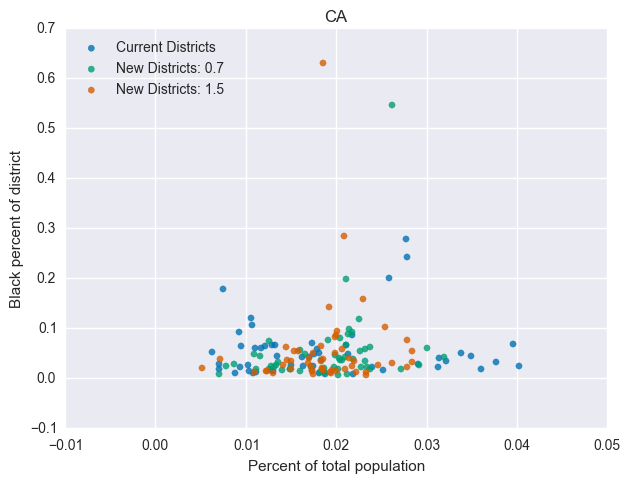
\includegraphics[width=4.5in]{../analysis/CA/analysis_scatter2.png}
\end{figure}

\clearpage
\newpage

\subsection{Alabama}
\begin{figure}[htb!] \centering
\caption{ Current Districts }
\includegraphics[width=5in,height=3in,keepaspectratio]{../maps/AL/static/0_before.png}
\caption{ New Districts (Black Param = 0) }
\includegraphics[width=5in,height=3in,keepaspectratio]{../maps/AL/static/0_after.png}
\caption{ New Districts (Black Param = 1) }
\includegraphics[width=5in,height=3in,keepaspectratio]{../maps/AL/static/1_after.png}
\end{figure}

\clearpage
\newpage

\begin{figure}[htb!] \centering
\caption{ Demographics: black population }
\includegraphics[width=4.5in]{../analysis/AL/analysis_scatter.png}
\caption{ Politics: democratic population (placeholder)}
\includegraphics[width=4.5in]{../analysis/AL/analysis_scatter2.png}
\end{figure}

\clearpage
\newpage

\subsection{Illinois}
\begin{figure}[htb!] \centering
\caption{ Current Districts }
\includegraphics[width=5in,height=3in,keepaspectratio]{../maps/IL/static/0_before.png}
\caption{ New Districts (Black Param = 0) }
\includegraphics[width=5in,height=3in,keepaspectratio]{../maps/IL/static/0_after.png}
\caption{ New Districts (Black Param = 1) }
\includegraphics[width=5in,height=3in,keepaspectratio]{../maps/IL/static/1_after.png}
\end{figure}

\clearpage
\newpage

\begin{figure}[htb!] \centering
\caption{ Demographics: black population }
\includegraphics[width=4.5in]{../analysis/IL/analysis_scatter.png}
\caption{ Politics: democratic population (placeholder)}
\includegraphics[width=4.5in]{../analysis/IL/analysis_scatter2.png}
\end{figure}

\clearpage
\newpage

\subsection{Georgia}
\begin{figure}[htb!] \centering
\caption{ Current Districts }
\includegraphics[width=5in,height=3in,keepaspectratio]{../maps/GA/static/0_before.png}
\caption{ New Districts (Black Param = 0) }
\includegraphics[width=5in,height=3in,keepaspectratio]{../maps/GA/static/0_after.png}
\caption{ New Districts (Black Param = 1) }
\includegraphics[width=5in,height=3in,keepaspectratio]{../maps/GA/static/1_after.png}
\end{figure}

\clearpage
\newpage

\begin{figure}[htb!] \centering
\caption{ Demographics: black population }
\includegraphics[width=4.5in]{../analysis/GA/analysis_scatter.png}
\caption{ Politics: democratic population (placeholder)}
\includegraphics[width=4.5in]{../analysis/GA/analysis_scatter2.png}
\end{figure}

\clearpage
\newpage

\subsection{Indiana}
\begin{figure}[htb!] \centering
\caption{ Current Districts }
\includegraphics[width=5in,height=3in,keepaspectratio]{../maps/IN/static/0_before.png}
\caption{ New Districts (Black Param = 0) }
\includegraphics[width=5in,height=3in,keepaspectratio]{../maps/IN/static/0_after.png}
\caption{ New Districts (Black Param = 1) }
\includegraphics[width=5in,height=3in,keepaspectratio]{../maps/IN/static/1_after.png}
\end{figure}

\clearpage
\newpage

\begin{figure}[htb!] \centering
\caption{ Demographics: black population }
\includegraphics[width=4.5in]{../analysis/IN/analysis_scatter.png}
\caption{ Politics: democratic population (placeholder)}
\includegraphics[width=4.5in]{../analysis/IN/analysis_scatter2.png}
\end{figure}

\clearpage
\newpage

\subsection{Iowa}
\begin{figure}[htb!] \centering
\caption{ Current Districts }
\includegraphics[width=5in,height=3in,keepaspectratio]{../maps/IA/static/0_before.png}
\caption{ New Districts (Black Param = 0) }
\includegraphics[width=5in,height=3in,keepaspectratio]{../maps/IA/static/0_after.png}
\caption{ New Districts (Black Param = 1) }
\includegraphics[width=5in,height=3in,keepaspectratio]{../maps/IA/static/1_after.png}
\end{figure}

\clearpage
\newpage

\begin{figure}[htb!] \centering
\caption{ Demographics: black population }
\includegraphics[width=4.5in]{../analysis/IA/analysis_scatter.png}
\caption{ Politics: democratic population (placeholder)}
\includegraphics[width=4.5in]{../analysis/IA/analysis_scatter2.png}
\end{figure}

\clearpage
\newpage

\subsection{Massachusetts}
\begin{figure}[htb!] \centering
\caption{ Current Districts }
\includegraphics[width=5in,height=3in,keepaspectratio]{../maps/MA/static/0_before.png}
\caption{ New Districts (Black Param = 0) }
\includegraphics[width=5in,height=3in,keepaspectratio]{../maps/MA/static/0_after.png}
\caption{ New Districts (Black Param = 1) }
\includegraphics[width=5in,height=3in,keepaspectratio]{../maps/MA/static/1_after.png}
\end{figure}

\clearpage
\newpage

\begin{figure}[htb!] \centering
\caption{ Demographics: black population }
\includegraphics[width=4.5in]{../analysis/MA/analysis_scatter.png}
\caption{ Politics: democratic population (placeholder)}
\includegraphics[width=4.5in]{../analysis/MA/analysis_scatter2.png}
\end{figure}

\clearpage
\newpage

\subsection{Arizona}
\begin{figure}[htb!] \centering
\caption{ Current Districts }
\includegraphics[width=5in,height=3in,keepaspectratio]{../maps/AZ/static/0_before.png}
\caption{ New Districts (Black Param = 0) }
\includegraphics[width=5in,height=3in,keepaspectratio]{../maps/AZ/static/0_after.png}
\caption{ New Districts (Black Param = 1) }
\includegraphics[width=5in,height=3in,keepaspectratio]{../maps/AZ/static/1_after.png}
\end{figure}

\clearpage
\newpage

\begin{figure}[htb!] \centering
\caption{ Demographics: black population }
\includegraphics[width=4.5in]{../analysis/AZ/analysis_scatter.png}
\caption{ Politics: democratic population (placeholder)}
\includegraphics[width=4.5in]{../analysis/AZ/analysis_scatter2.png}
\end{figure}

\clearpage
\newpage

\subsection{Connecticut}
\begin{figure}[htb!] \centering
\caption{ Current Districts }
\includegraphics[width=5in,height=3in,keepaspectratio]{../maps/CT/static/0_before.png}
\caption{ New Districts (Black Param = 0) }
\includegraphics[width=5in,height=3in,keepaspectratio]{../maps/CT/static/0_after.png}
\caption{ New Districts (Black Param = 1) }
\includegraphics[width=5in,height=3in,keepaspectratio]{../maps/CT/static/1_after.png}
\end{figure}

\clearpage
\newpage

\begin{figure}[htb!] \centering
\caption{ Demographics: black population }
\includegraphics[width=4.5in]{../analysis/CT/analysis_scatter.png}
\caption{ Politics: democratic population (placeholder)}
\includegraphics[width=4.5in]{../analysis/CT/analysis_scatter2.png}
\end{figure}

\clearpage
\newpage

\subsection{Maryland}
\begin{figure}[htb!] \centering
\caption{ Current Districts }
\includegraphics[width=5in,height=3in,keepaspectratio]{../maps/MD/static/0_before.png}
\caption{ New Districts (Black Param = 0) }
\includegraphics[width=5in,height=3in,keepaspectratio]{../maps/MD/static/0_after.png}
\caption{ New Districts (Black Param = 1) }
\includegraphics[width=5in,height=3in,keepaspectratio]{../maps/MD/static/1_after.png}
\end{figure}

\clearpage
\newpage

\begin{figure}[htb!] \centering
\caption{ Demographics: black population }
\includegraphics[width=4.5in]{../analysis/MD/analysis_scatter.png}
\caption{ Politics: democratic population (placeholder)}
\includegraphics[width=4.5in]{../analysis/MD/analysis_scatter2.png}
\end{figure}

\clearpage
\newpage

\subsection{Oklahoma}
\begin{figure}[htb!] \centering
\caption{ Current Districts }
\includegraphics[width=5in,height=3in,keepaspectratio]{../maps/OK/static/0_before.png}
\caption{ New Districts (Black Param = 0) }
\includegraphics[width=5in,height=3in,keepaspectratio]{../maps/OK/static/0_after.png}
\caption{ New Districts (Black Param = 1) }
\includegraphics[width=5in,height=3in,keepaspectratio]{../maps/OK/static/1_after.png}
\end{figure}

\clearpage
\newpage

\begin{figure}[htb!] \centering
\caption{ Demographics: black population }
\includegraphics[width=4.5in]{../analysis/OK/analysis_scatter.png}
\caption{ Politics: democratic population (placeholder)}
\includegraphics[width=4.5in]{../analysis/OK/analysis_scatter2.png}
\end{figure}

\clearpage
\newpage

\subsection{Ohio}
\begin{figure}[htb!] \centering
\caption{ Current Districts }
\includegraphics[width=5in,height=3in,keepaspectratio]{../maps/OH/static/0_before.png}
\caption{ New Districts (Black Param = 0) }
\includegraphics[width=5in,height=3in,keepaspectratio]{../maps/OH/static/0_after.png}
\caption{ New Districts (Black Param = 1) }
\includegraphics[width=5in,height=3in,keepaspectratio]{../maps/OH/static/1_after.png}
\end{figure}

\clearpage
\newpage

\begin{figure}[htb!] \centering
\caption{ Demographics: black population }
\includegraphics[width=4.5in]{../analysis/OH/analysis_scatter.png}
\caption{ Politics: democratic population (placeholder)}
\includegraphics[width=4.5in]{../analysis/OH/analysis_scatter2.png}
\end{figure}

\clearpage
\newpage

\subsection{Missouri}
\begin{figure}[htb!] \centering
\caption{ Current Districts }
\includegraphics[width=5in,height=3in,keepaspectratio]{../maps/MO/static/0_before.png}
\caption{ New Districts (Black Param = 0) }
\includegraphics[width=5in,height=3in,keepaspectratio]{../maps/MO/static/0_after.png}
\caption{ New Districts (Black Param = 1) }
\includegraphics[width=5in,height=3in,keepaspectratio]{../maps/MO/static/1_after.png}
\end{figure}

\clearpage
\newpage

\begin{figure}[htb!] \centering
\caption{ Demographics: black population }
\includegraphics[width=4.5in]{../analysis/MO/analysis_scatter.png}
\caption{ Politics: democratic population (placeholder)}
\includegraphics[width=4.5in]{../analysis/MO/analysis_scatter2.png}
\end{figure}

\clearpage
\newpage

\subsection{Minnesota}
\begin{figure}[htb!] \centering
\caption{ Current Districts }
\includegraphics[width=5in,height=3in,keepaspectratio]{../maps/MN/static/0_before.png}
\caption{ New Districts (Black Param = 0) }
\includegraphics[width=5in,height=3in,keepaspectratio]{../maps/MN/static/0_after.png}
\caption{ New Districts (Black Param = 1) }
\includegraphics[width=5in,height=3in,keepaspectratio]{../maps/MN/static/1_after.png}
\end{figure}

\clearpage
\newpage

\begin{figure}[htb!] \centering
\caption{ Demographics: black population }
\includegraphics[width=4.5in]{../analysis/MN/analysis_scatter.png}
\caption{ Politics: democratic population (placeholder)}
\includegraphics[width=4.5in]{../analysis/MN/analysis_scatter2.png}
\end{figure}

\clearpage
\newpage

\subsection{Kansas}
\begin{figure}[htb!] \centering
\caption{ Current Districts }
\includegraphics[width=5in,height=3in,keepaspectratio]{../maps/KS/static/0_before.png}
\caption{ New Districts (Black Param = 0) }
\includegraphics[width=5in,height=3in,keepaspectratio]{../maps/KS/static/0_after.png}
\caption{ New Districts (Black Param = 1) }
\includegraphics[width=5in,height=3in,keepaspectratio]{../maps/KS/static/1_after.png}
\end{figure}

\clearpage
\newpage

\begin{figure}[htb!] \centering
\caption{ Demographics: black population }
\includegraphics[width=4.5in]{../analysis/KS/analysis_scatter.png}
\caption{ Politics: democratic population (placeholder)}
\includegraphics[width=4.5in]{../analysis/KS/analysis_scatter2.png}
\end{figure}

\clearpage
\newpage

\subsection{Mississippi}
\begin{figure}[htb!] \centering
\caption{ Current Districts }
\includegraphics[width=5in,height=3in,keepaspectratio]{../maps/MS/static/0_before.png}
\caption{ New Districts (Black Param = 0) }
\includegraphics[width=5in,height=3in,keepaspectratio]{../maps/MS/static/0_after.png}
\caption{ New Districts (Black Param = 1) }
\includegraphics[width=5in,height=3in,keepaspectratio]{../maps/MS/static/1_after.png}
\end{figure}

\clearpage
\newpage

\begin{figure}[htb!] \centering
\caption{ Demographics: black population }
\includegraphics[width=4.5in]{../analysis/MS/analysis_scatter.png}
\caption{ Politics: democratic population (placeholder)}
\includegraphics[width=4.5in]{../analysis/MS/analysis_scatter2.png}
\end{figure}

\clearpage
\newpage

\subsection{South Carolina}
\begin{figure}[htb!] \centering
\caption{ Current Districts }
\includegraphics[width=5in,height=3in,keepaspectratio]{../maps/SC/static/0_before.png}
\caption{ New Districts (Black Param = 0) }
\includegraphics[width=5in,height=3in,keepaspectratio]{../maps/SC/static/0_after.png}
\caption{ New Districts (Black Param = 1) }
\includegraphics[width=5in,height=3in,keepaspectratio]{../maps/SC/static/1_after.png}
\end{figure}

\clearpage
\newpage

\begin{figure}[htb!] \centering
\caption{ Demographics: black population }
\includegraphics[width=4.5in]{../analysis/SC/analysis_scatter.png}
\caption{ Politics: democratic population (placeholder)}
\includegraphics[width=4.5in]{../analysis/SC/analysis_scatter2.png}
\end{figure}

\clearpage
\newpage

